% ============================================================================
% GALOSH — IEEE SPL 版 日本語（内容確認用。投稿は英語版 galosh_spl.tex）
% Build: tectonic galosh_spl_ja.tex   (XeTeX + xeCJK)
% ============================================================================
\documentclass[journal]{IEEEtran}
\usepackage{booktabs}
\usepackage{graphicx}
\usepackage{amsmath,amssymb}
\usepackage[hidelinks]{hyperref}
% CJK: tectonic/XeTeX はフォント指定が無いと日本語グリフを黙って落とす
\usepackage{xeCJK}
\setCJKmainfont[BoldFont={Yu Gothic Bold}]{Yu Mincho}
\setCJKsansfont{Yu Gothic}
\setCJKmonofont{MS Gothic}

\begin{document}

\title{GALOSH: 並列フレンドリな局所シュリンケージによる\\
Raw Bayer・sRGB 画像のブラインド・学習不要デノイジング}

\author{Yoshiro~Sato%
\thanks{本稿記載の手法を対象とする米国仮特許出願済み（App.\ No.\ 64/058,343、
2026 年 5 月 6 日）。}%
\thanks{コードと再現可能ベンチマーク:
\texttt{https://github.com/luxgrain/GALOSH}。全データセットの完全な表・ISO 帯別
内訳・速度検証を含む拡張版は arXiv プレプリント~\cite{galosharxiv}。}}

\maketitle

\begin{abstract}
BM3D や non-local means のような学習不要の古典的デノイザは、その強さの多くを
「探索」--- 並列化しにくく固定レイテンシ実装を阻む内容依存のブロックマッチング
--- に負っている。本稿では探索を丸ごと取り除いた再設計 GALOSH（Generalized
Anscombe LOcal SHrinkage）を提案する: 画像ごとのブラインド Poisson--Gaussian
ノイズ推定、一般化 Anscombe 変換、輝度の 2 パス局所 Walsh--Hadamard
シュリンケージ、輝度ガイドの色差局所回帰 --- 知覚的に異なる 2 つのノイズ成分に
対する意図的に異なる 2 演算子である。全ステージが局所的・データ非依存・規則的で
あり、一つのコアが raw Bayer モザイクと sRGB/YUV 画像の両方を扱う。実ノイズ 4
ベンチマーク（SIDD Medium と RawNIND の raw・sRGB）で、GALOSH は比較した
blind・training-free 手法の中で一貫して最良 --- オラクルのノイズレベルを与えた
BM3D/NLM 系すら上回る --- でありながら、同一 GPU 上で学習ベースラインの
$7\times$--$650\times$ 高速に走り、通常の CPU でも実用速度で動く。固定された
構造は固定小数点ストリーミングハードウェアへの写像を意図して設計されており、
動作する INT16 実現がこれを裏付ける。
\end{abstract}

\begin{IEEEkeywords}
Image denoising, blind denoising, variance stabilization, Walsh--Hadamard
transform, fixed-point arithmetic.
\end{IEEEkeywords}

\section{はじめに}
画像デノイジングには二つの系譜がある。古典的な学習不要手法 ---
BM3D~\cite{bm3d} と non-local means~\cite{nlm} --- はデータ不要でセンサを横断して
一般化するが、既知のノイズレベルを前提とし、その品質を内容依存の「探索」で
買っている: ブロックマッチングと近傍重み付けの不規則なメモリアクセスと
データ依存制御フローは、ベクトル化・GPU 占有率・固定レイテンシ予算のいずれにも
抵抗する。学習ベースの手法は学習したドメインでは優れた品質に達するが、学習
ペアを必要とし、ピクセルあたり数万 MAC を要し、学習分布の外では --- ときに
壊滅的に --- 劣化する（本稿でも実測される）。BM3D/NLM 以外にも古典系には
低ランクパッチモデル（WNNM~\cite{wnnm}）、パッチ事前分布最適化
（EPLL~\cite{epll}）、学習辞書（K-SVD~\cite{ksvd}）、ブラインドの Noise Clinic
パイプライン~\cite{noiseclinic}があるが、いずれも同様に探索ないし最適化が重く、
本稿の比較では最も広く再現されている代表として BM3D/NLM（CFA 対応・カラー変種を
含む）を採用する。

本稿の問いはこうである: 探索を設計によって取り除いたとき、古典系の品質は
どこまで残るか？GALOSH は、全ステージが局所的・規則的・データ非依存の
パイプラインで答える: ノイズモデルは画像自体からブラインドに推定され~\cite{foi}、
一般化 Anscombe 変換（GAT）が単一のグローバル閾値を画面全体で有効にし、輝度は
Walsh--Hadamard 分解上の 2 パス局所シュリンケージ（BayesShrink~\cite{bayesshrink}
のパイロット + 経験的 Wiener パス、BM3D の 2 段構成と同様）で、色差は輝度ガイドの
局所線形回帰（bilateral カーネルを持つ LOESS~\cite{loess}、guided/joint-bilateral
系~\cite{kopf,guidedfilter}の伝統に連なる）でデノイズされる。輝度/色差分離は
意図的である: 輝度ノイズは粒状感として現れテクスチャと共存できるが、色差ノイズは
決して許容されない色むらとして現れるため、2 つの経路は異なる攻撃性の異なる
演算子を使い、独立した強度制御を公開する。同じコアが 2 つの薄い前段に仕える:
Bayer モザイク上の \textbf{GALOSH-RAW}（各クワッドの $2{\times}2$
Walsh--Hadamard 変換が輝度/色差分離を与える）とレンダリング済み sRGB 画像上の
\textbf{GALOSH-YUV/RGB}（線形光 BT.709 変換が同じ分離を与える）。本稿の主張は
単一の構成要素ではなく、それらを探索不要・完全ブラインド・2 ドメインの、どの
画像のどのピクセルでも計算グラフが固定されたパイプラインへ合成したことにある。

\section{手法}
\subsection{共有コア}
\paragraph{ブラインドノイズ推定} Poisson--Gaussian モデル
$\mathrm{Var}[x]=\alpha\,\mathbb{E}[x]+\sigma^2$ を、重なり合うブロック上の局所
Laplacian 分散対局所平均のロバスト回帰（Foi 型推定器~\cite{foi}）でノイズ
フレームのみからフィットし、キャリブレーションデータもオラクルもなしに画像
ごとの $(\alpha,\sigma^2)$ を得る。

\paragraph{分散安定化} GAT
$f(x)=\tfrac{2}{\alpha}\sqrt{\alpha x+\tfrac{3}{8}\alpha^2+\sigma^2}$ が信号依存
ノイズをほぼ単位分散へ写し、単一のグローバル閾値がフレーム全体で有効になる。
出力には厳密な不偏逆~\cite{makitalo}を適用する。高域残差のチャネル別中央絶対
偏差（MAD）が残差スケールを与える。

\paragraph{輝度: 2 パス局所シュリンケージ（LOSH）} 輝度は、stride-1 サイクル
スピンの下で重なり合う $8{\times}8$ Walsh--Hadamard ブロック上でデノイズされる:
パス 1 はロバスト BayesShrink 閾値~\cite{bayesshrink}でパイロットを作り、パス 2
はパイロット係数から計算した経験的 Wiener ゲインを適用し、重なりブロックは
窓付き overlap-add で再結合される。これは BM3D の「探索された」ブロック上の協調
3-D スタックを、密なサイクルスピン局所変換で置き換えるもの --- 内容依存性を
すべて取り除く一手である。

\paragraph{色差: 輝度ガイド回帰} 各色差プレーンは、デノイズ済み輝度上の 1 次
局所重み付き回帰（bilateral カーネルを持つ Y ガイド LOESS~\cite{loess}、guided
filter~\cite{guidedfilter,kopf}と同趣旨）でデノイズされる: 各局所窓内でカーネル
重みが空間距離と輝度類似度を組み合わせ、MAP 正則化された傾き/切片が輝度構造を
再彩色する。マルチスケール残差ピラミッドが同じ演算子を粗い色むらへ拡張する。
再構成された色差は局所入力色差レンジへクランプされる（「デノイザは入力にない色を
発明してはならない」）。2 つの経路は独立した強度 $s_L,s_C$ を公開する。全
ベンチマークは固定デフォルトを使う。

\subsection{ドメイン前段}
\paragraph{GALOSH-RAW} Bayer モザイク上で直接動く: ブラインドフィットと GAT の
後、CFA 対応の無彩色ダークリファレンス（無彩色フロアの IRLS 推定）を減算し、
stride-1 サイクルスピン $2{\times}2$ Walsh--Hadamard 変換が各 Bayer クワッドを
1 つのフル解像度輝度プレーンと 3 つの半解像度色差プレーンへ写す。色差は半解像度
でデノイズされ、局所 $2{\times}2$ 入力ハルへのアンチリンギングクランプ付きの
輝度ガイド joint-bilateral EWA-jinc アップサンプリングでフル解像度へ戻される。
逆 WHT、ダーク復元、厳密逆 GAT により、任意のデモザイク後段に渡せるデノイズ
済み Bayer フレームが得られる。

\paragraph{GALOSH-YUV/RGB} レンダリング済み sRGB を受け付ける: 逆ガンマで線形光
へ、フルレンジ BT.709 YCbCr へ変換する。Y は GAT + 2 パス LOSH を
（レンダリング後のノイズもトーンカーブを通して信号依存のままであり、GAT が一次
近似でそれを吸収する）、Cb/Cr はフル解像度でガイド回帰を受ける。同じ局所色差
レンジクランプを適用し、出力は $[0,1]$ へクランプされる。

\section{実験}
\paragraph{設定} raw ドメイン: \textbf{SIDD Medium}~\cite{sidd}（フル解像度
スマートフォン Bayer 80 枚）と \textbf{RawNIND}~\cite{rawnind}（カメラ横断
$512^2$ 実ノイズクロップ 1493 枚）。sRGB ドメイン: 同じ 2 セットの sRGB 版
（SIDD はフル ${\sim}15.8$\,MP フレーム）。\emph{すべてブラインドで走る}:
クリーン/ノイズペアなし、画像ごとのノイズオラクルなし。古典的ベースラインは
入力から $\sigma$ を推定し、GALOSH は自前のブラインドフィットを、学習ベース
ラインは公開されている実ノイズ学習済み重みを使う。忠実度（PSNR/SSIM）は各
ネイティブドメインで、知覚指標（LPIPS~\cite{lpips}）は sRGB 上で計算する。
フルフレーム sRGB では学習ベースラインはタイル推論で走らせ、LPIPS は全手法で
同一の $1024^2$ タイル格子上の平均として報告する --- この解像度でのメモリと
指標実装の制約による統一プロトコルである。ベースラインは設計上ドメインごとに
適切なものを使う: raw では CFA 対応手法（BM3D-CFA、NLM-CFA、その VST 前段
アブレーション、raw 学習の Blind2Unblind~\cite{b2u}）、sRGB ではカラー画像手法
（CBM3D、Color-NLM、self-guided filter、sRGB 学習の NAFNet~\cite{nafnet}、
Restormer~\cite{restormer}、SCUNet~\cite{scunet}）。

\begin{table}[t]
\centering
\caption{raw 領域ブラインド・デノイジング。全手法ブラインド。太字 /
\underline{下線} = blind・training-free 手法中の最良 / 2 位。Blind2Unblind は
学習済みの上限参照。DISTS/NIQE と画像あたり時間を含む完全な表は拡張版
~\cite{galosharxiv}。}
\label{tab:raw}
\setlength{\tabcolsep}{3pt}
\footnotesize
\begin{tabular}{l ccc ccc}
\toprule
 & \multicolumn{3}{c}{SIDD Medium（フル 80 枚）} & \multicolumn{3}{c}{RawNIND（1493 クロップ）}\\
\cmidrule(lr){2-4}\cmidrule(lr){5-7}
Method & PSNR$\uparrow$ & SSIM$\uparrow$ & LPIPS$\downarrow$ & PSNR$\uparrow$ & SSIM$\uparrow$ & LPIPS$\downarrow$\\
\midrule
GALOSH FP32   & \textbf{48.13} & \textbf{0.9883} & \textbf{0.2030} & \underline{30.49} & \underline{0.7908} & \textbf{0.2395}\\
GALOSH INT16  & \underline{47.42} & \underline{0.9881} & \textbf{0.2030} & 30.17 & 0.7860 & \underline{0.2453}\\
VST+GALOSH    & 44.35 & 0.9765 & 0.2132 & \textbf{30.63} & \textbf{0.8163} & 0.2481\\
VST+BM3D-CFA  & 45.96 & 0.9851 & 0.2932 & 30.07 & 0.7792 & 0.4320\\
VST+NLM-CFA   & 40.36 & 0.9679 & 0.4048 & 29.03 & 0.7649 & 0.5452\\
BM3D-CFA      & 46.74 & 0.9862 & 0.2725 & 30.28 & 0.7848 & 0.4268\\
NLM-CFA       & 42.32 & 0.9729 & 0.3791 & 29.54 & 0.7735 & 0.5190\\
\midrule
Blind2Unblind & 49.07 & 0.9924 & 0.1169 & 30.68 & 0.7932 & 0.2215\\
\bottomrule
\end{tabular}
\end{table}

\begin{table}[t]
\centering
\caption{SIDD Medium sRGB（80 シーン、フル ${\sim}15.8$\,MP フレーム）における
sRGB 領域ブラインド・デノイジング。学習済みネットワークは上限参照（NAFNet と
Restormer は SIDD で学習）。}
\label{tab:srgb}
\setlength{\tabcolsep}{4pt}
\footnotesize
\begin{tabular}{l ccc}
\toprule
Method & PSNR$\uparrow$ & SSIM$\uparrow$ & LPIPS$\downarrow$\\
\midrule
Noisy input     & 25.69 & 0.424 & 0.790\\
GALOSH-YUV      & \textbf{35.01} & \textbf{0.837} & \textbf{0.314}\\
CBM3D           & 27.09 & 0.492 & 0.721\\
Color-NLM       & \underline{28.92} & \underline{0.656} & \underline{0.534}\\
Guided filter   & 27.43 & 0.523 & 0.687\\
\midrule
NAFNet-SIDD     & 41.94 & 0.942 & 0.167\\
Restormer-SIDD  & 40.94 & 0.935 & 0.181\\
SCUNet-real     & 36.09 & 0.902 & 0.252\\
\bottomrule
\end{tabular}
\end{table}

\begin{figure*}[t]
\centering
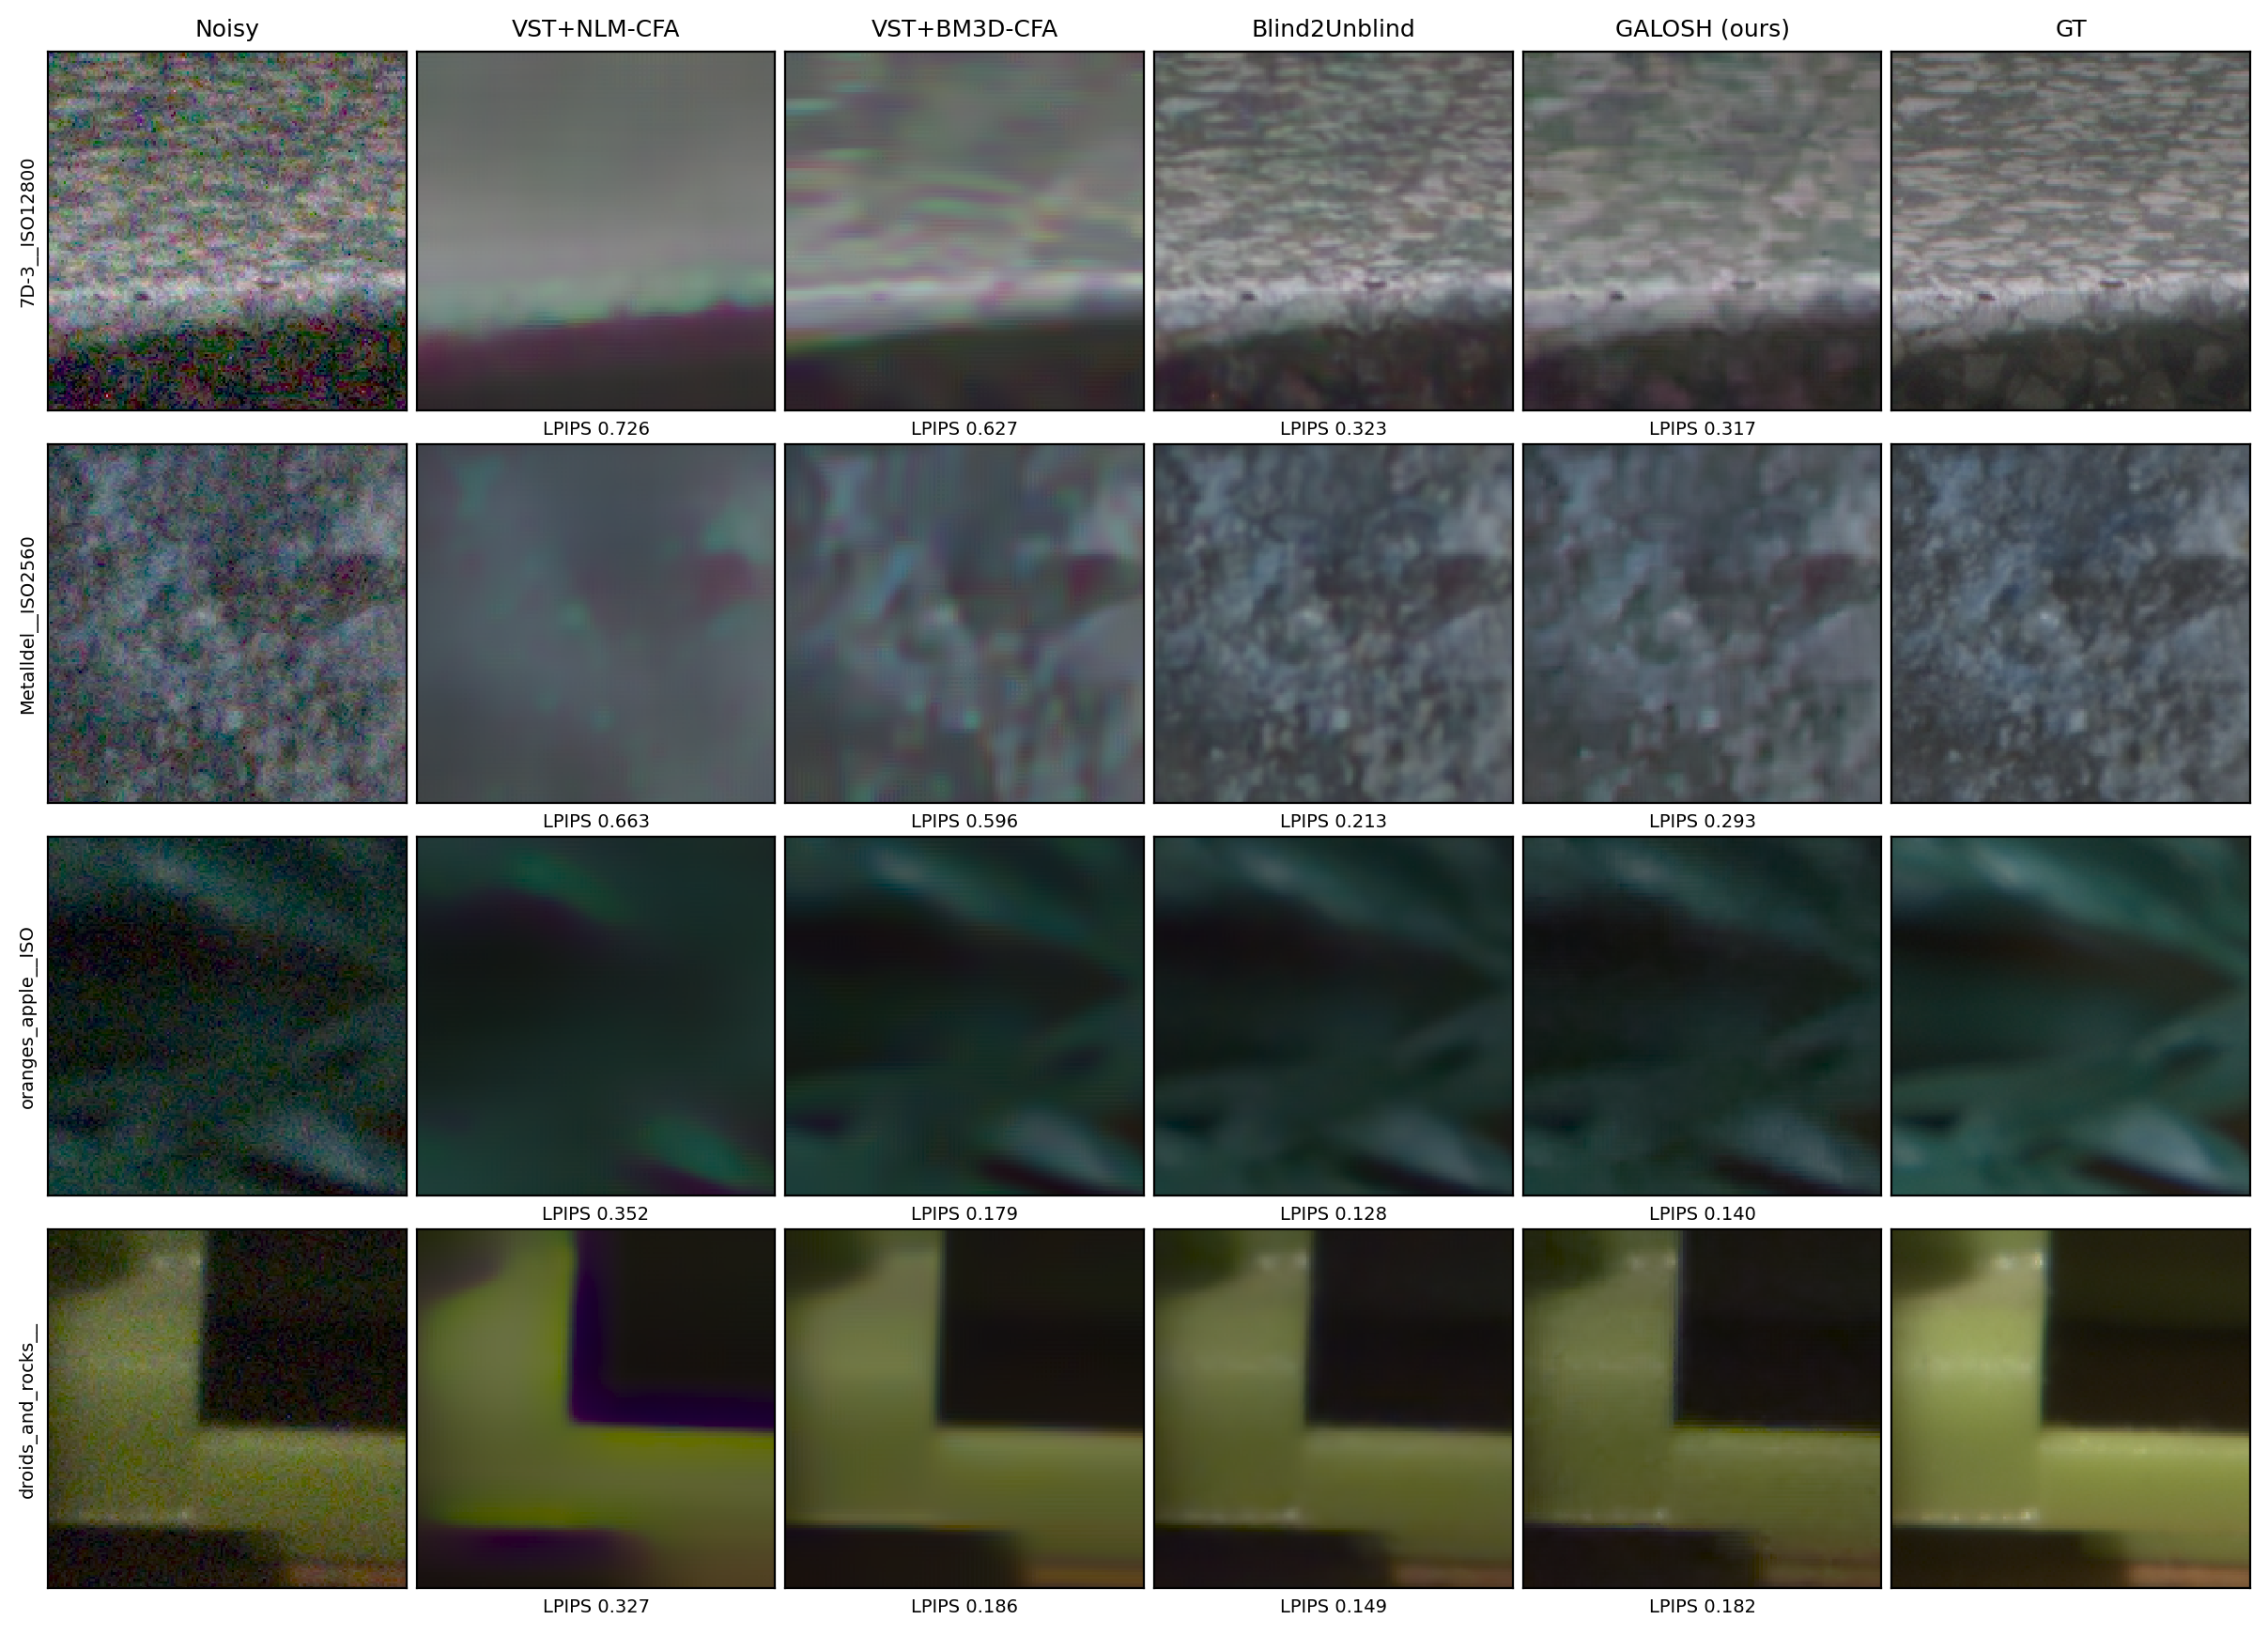
\includegraphics[width=0.92\textwidth]{../qualitative_rawnind.png}
\caption{raw ドメイン、RawNIND。列: Noisy / VST+NLM-CFA / VST+BM3D-CFA /
Blind2Unblind（学習済み） / \textbf{GALOSH（提案、blind）} / GT。画像ごとの
LPIPS（$\downarrow$）付き。古典的ベースラインにはノイズ考慮の VST 前段を与えて
おり、GALOSH は完全ブラインドである。}
\label{fig:qual}
\end{figure*}

\paragraph{raw ドメイン} 表~\ref{tab:raw}: 比較した blind・training-free 手法の
中で GALOSH は両データセットの知覚指標で大差の最良（LPIPS $0.203$/$0.240$ 対
BM3D/NLM 系の $0.27$--$0.55$、共有 VST 前段の有無によらず）であり、PSNR/SSIM
でも競争力がある。\emph{学習済み}の Blind2Unblind 参照に対しては、RawNIND で
知覚ギャップの大半を学習なしで詰める（LPIPS $0.240$ 対 $0.222$）。VST
アブレーション行が優位性の源泉を分離する: 古典的ベースラインに GALOSH 自身の
分散安定化前段を与えても改善はわずかであり、ギャップの正体はノイズモデルでは
なく探索不要の局所シュリンケージアーキテクチャである。さらに RawNIND の最も
ノイジーなサブセット（ISO${\geq}6400$）で、CBM3D と Color-NLM にグラウンド
トゥルースから計算したオラクルを含む 3 種類の $\sigma$ を与えて再実行しても、
両者は完全ブラインドの GALOSH を下回る --- 優位はアルゴリズムであり、推定では
ない。

\paragraph{sRGB ドメイン} 表~\ref{tab:srgb}: フルフレーム SIDD sRGB で GALOSH
は比較したブラインド古典的手法に決定的に勝つ（$+6$--$8$\,dB PSNR、LPIPS は
ほぼ半分）: 空間相関を持つ信号依存のレンダリングノイズは、彼らの $\sigma$
推定器と白色ノイズ仮定の両方を打ち破る。SIDD 学習ネットワークは自らのドメイン
では明確に先行し（NAFNet $41.94$\,dB）--- 上限参照として正直に報告する。
クロスドメインの RawNIND sRGB では集計がほぼクリーンな低 ISO シーンに支配され
る; デノイジングが効く高 ISO 帯では GALOSH は古典的ベースラインを明確に上回り、
学習済みネットワークがやや上回る（$+0.3$--$0.7$\,dB）。SIDD 学習ネットワークの
一つは暗部 37 シーンで数値発散する（クリップ前のネットワーク生出力が
$\pm10^3$ に達する）が、GALOSH を含む他の全ベースラインは同じ入力で安定である
--- 固定された学習不要計算のロバスト性の利得である（完全な表は
~\cite{galosharxiv}）。

\paragraph{速度} 探索不要性は直接効く。単一 GPU（RTX 4070\,Ti）で GALOSH は
16-MP raw フレームを $0.76$\,s（Blind2Unblind の $5.6$\,s に対し $7\times$）、
$15.8$-MP sRGB フレームを $0.87$\,s（比較したネットワークの $13.5$--$565$\,s
に対し $15$--$650\times$）でデノイズし、GPU カーネルパイプラインは 1080p を
$18.2$\,ms、4K を $46$\,ms で走る。1080p の単一 CPU コアでは $1.38$\,s 対
NLM-CFA/BM3D-CFA の $3.21$/$6.33$\,s --- 比較中で唯一、両プラットフォームで
最速の手法である（計測プロトコルと完全な表は~\cite{galosharxiv}）。

\section{並列・固定小数点への写像}
探索を取り除くと計算グラフが固定されるため、ハードウェア実装を主張することなく
その帰結を定量化できる。raw パイプライン全体の計測で、GALOSH のコストはピクセル
あたり約 $3.4$k 積和 + 約 $140$ LUT/特殊演算で、解像度非依存 --- BM3D/NLM の
$3.9$--$6.4\times$ 下、学習ベースラインの $18$--$360\times$ 下であり、全域で
局所的・データ非依存のアクセスパターンを持つ。シュリンケージコアは純 INT16
ストレージ / INT32 アキュムレートの固定小数点形式を持つ: INT32 ストレージでは
GPU ストリーミング実装は INT32 CPU 参照と end-to-end で bit-exact に一致し
（フルフレームで検証済み）、ラインバッファを INT16 ストレージ形式（輝度 Q10.5、
クロマ Q6.9）に狭めても両者は near-lossless（$\approx$58--65\,dB PSNR ---
まさにストレージ量子化そのもの）であり、INT16 の品質自体は FP32 の
$0.1$--$0.7$\,dB 以内である（表~\ref{tab:raw}）。出荷パスに 64 bit 演算は
不要である。MAC アレイのスループットモデルによれば、ピクセルあたり演算数は
$0.5$--$1$\,TMAC/s の固定機能演算予算の下で 1080p--4K 級ストリーミングと
両立し、オンチップ状態は最大垂直カーネルのラインバッファで抑えられる
（1080p・INT16 で ${\sim}200$\,KB）。これらは設計特性 ---「固定小数点
ストリーミングハードウェアへ自然に写像するよう設計されている」--- として提示
するのであって、完成した ISP 実装としてではない。

\section{結論}
古典的デノイジングから探索を取り除く --- ブロックマッチングを分散安定化された
サイクルスピン局所シュリンケージと輝度ガイド色差回帰で置き換える --- ことで、
古典系の品質は保たれ（オラクル条件下でも比較した古典系を上回る）、一つの
学習不要コアで 2 ドメインへ拡張され、高速になる: 同一 GPU で学習ベースラインの
$7\times$--$650\times$ 先、通常の CPU でも実用的、そして固定小数点ストリーミング
ハードウェアへの写像を意図した設計である。

\begin{thebibliography}{21}\small
\bibitem{bm3d} K.~Dabov, A.~Foi, V.~Katkovnik, and K.~Egiazarian, ``Image
denoising by sparse 3-D transform-domain collaborative filtering,'' \emph{IEEE
TIP}, 2007.
\bibitem{nlm} A.~Buades, B.~Coll, and J.-M.~Morel, ``A non-local algorithm for
image denoising,'' \emph{CVPR}, 2005.
\bibitem{foi} A.~Foi, M.~Trimeche, V.~Katkovnik, and K.~Egiazarian,
``Practical Poissonian-Gaussian noise modeling and fitting for single-image
raw-data,'' \emph{IEEE TIP}, 2008.
\bibitem{makitalo} M.~Makitalo and A.~Foi, ``Optimal inversion of the
generalized Anscombe transformation for Poisson-Gaussian noise,'' \emph{IEEE
TIP}, 2013.
\bibitem{bayesshrink} S.~G.~Chang, B.~Yu, and M.~Vetterli, ``Adaptive wavelet
thresholding for image denoising and compression,'' \emph{IEEE TIP}, 2000.
\bibitem{loess} W.~S.~Cleveland, ``Robust locally weighted regression and
smoothing scatterplots,'' \emph{JASA}, 1979.
\bibitem{kopf} J.~Kopf, M.~F.~Cohen, D.~Lischinski, and M.~Uyttendaele,
``Joint bilateral upsampling,'' \emph{ACM SIGGRAPH}, 2007.
\bibitem{guidedfilter} K.~He, J.~Sun, and X.~Tang, ``Guided image filtering,''
\emph{ECCV}, 2010.
\bibitem{wnnm} S.~Gu, L.~Zhang, W.~Zuo, and X.~Feng, ``Weighted nuclear norm
minimization with application to image denoising,'' \emph{CVPR}, 2014.
\bibitem{epll} D.~Zoran and Y.~Weiss, ``From learning models of natural image
patches to whole image restoration,'' \emph{ICCV}, 2011.
\bibitem{ksvd} M.~Elad and M.~Aharon, ``Image denoising via sparse and
redundant representations over learned dictionaries,'' \emph{IEEE TIP}, 2006.
\bibitem{noiseclinic} M.~Lebrun, M.~Colom, and J.-M.~Morel, ``The noise
clinic: A blind image denoising algorithm,'' \emph{IPOL}, 2015.
\bibitem{b2u} Z.~Wang et al., ``Blind2Unblind: Self-supervised image denoising
with visible blind spots,'' \emph{CVPR}, 2022.
\bibitem{nafnet} L.~Chen, X.~Chu, X.~Zhang, and J.~Sun, ``Simple baselines for
image restoration,'' \emph{ECCV}, 2022.
\bibitem{restormer} S.~W.~Zamir et al., ``Restormer: Efficient transformer for
high-resolution image restoration,'' \emph{CVPR}, 2022.
\bibitem{scunet} K.~Zhang et al., ``Practical blind image denoising via
Swin-Conv-UNet and data synthesis,'' \emph{Machine Intelligence Research},
2023.
\bibitem{sidd} A.~Abdelhamed, S.~Lin, and M.~S.~Brown, ``A high-quality
denoising dataset for smartphone cameras,'' \emph{CVPR}, 2018.
\bibitem{rawnind} B.~Brummer and C.~De~Vleeschouwer, ``Natural image noise
dataset,'' \emph{CVPRW}, 2019.
\bibitem{lpips} R.~Zhang, P.~Isola, A.~A.~Efros, E.~Shechtman, and O.~Wang,
``The unreasonable effectiveness of deep features as a perceptual metric,''
\emph{CVPR}, 2018.
\bibitem{galosharxiv} Y.~Sato, ``GALOSH: Blind, training-free denoising of raw
Bayer and sRGB images by parallel-friendly local shrinkage,'' arXiv preprint,
2026. % TODO: arXiv ID (2507.XXXXX) が出たら挿入
\end{thebibliography}

\end{document}
